%%
%% Copyright 2007, 2008, 2009 Elsevier Ltd
%%
%% This file is part of the 'Elsarticle Bundle'.
%% ---------------------------------------------
%%
%% It may be distributed under the conditions of the LaTeX Project Public
%% License, either version 1.2 of this license or (at your option) any
%% later version.  The latest version of this license is in
%%    http://www.latex-project.org/lppl.txt
%% and version 1.2 or later is part of all distributions of LaTeX
%% version 1999/12/01 or later.
%%
%% The list of all files belonging to the 'Elsarticle Bundle' is
%% given in the file `manifest.txt'.
%%

%% Template article for Elsevier's document class `elsarticle'
%% with numbered style bibliographic references
%% SP 2008/03/01

\documentclass[10pt]{elsarticle}

\usepackage{setspace}
\doublespacing
\usepackage[letterpaper, margin=1in]{geometry}
\usepackage{multirow}
\usepackage{array}
\usepackage{amsmath}
\usepackage{wrapfig}

%% Use the option review to obtain double line spacing
%% \documentclass[authoryear,preprint,review,12pt]{elsarticle}

%% Use the options 1p,twocolumn; 3p; 3p,twocolumn; 5p; or 5p,twocolumn
%% for a journal layout:
%% \documentclass[final,1p,times]{elsarticle}
%% \documentclass[final,1p,times,twocolumn]{elsarticle}
%% \documentclass[final,3p,times]{elsarticle}
%% \documentclass[final,3p,times,twocolumn]{elsarticle}
%% \documentclass[final,5p,times]{elsarticle}
%% \documentclass[final,5p,times,twocolumn]{elsarticle}

%% For including figures, graphicx.sty has been loaded in
%% elsarticle.cls. If you prefer to use the old commands
%% please give \usepackage{epsfig}

%% The amssymb package provides various useful mathematical symbols
\usepackage{amssymb}

\usepackage{subfigure}
%% The amsthm package provides extended theorem environments
%% \usepackage{amsthm}

%% The lineno packages adds line numbers. Start line numbering with
%% \begin{linenumbers}, end it with \end{linenumbers}. Or switch it on
%% for the whole article with \linenumbers.
%% \usepackage{lineno}
\usepackage{bm}
\usepackage{graphicx}
%\journal{Nuclear Physics B}
\newcolumntype{P}[1]{>{\centering\arraybackslash}p{#1}}
\newcolumntype{M}[1]{>{\centering\arraybackslash}m{#1}}
\begin{document}

\begin{frontmatter}

%% Title, authors and addresses

%% use the tnoteref command within \title for footnotes;
%% use the tnotetext command for theassociated footnote;
%% use the fnref command within \author or \address for footnotes;
%% use the fntext command for theassociated footnote;
%% use the corref command within \author for corresponding author footnotes;
%% use the cortext command for theassociated footnote;
%% use the ead command for the email address,
%% and the form \ead[url] for the home page:
%% \title{Title\tnoteref{label1}}
%% \tnotetext[label1]{}
%% \author{Name\corref{cor1}\fnref{label2}}
%% \ead{email address}
%% \ead[url]{home page}
%% \fntext[label2]{}
%% \cortext[cor1]{}
%% \address{Address\fnref{label3}}
%% \fntext[label3]{}

\title{GPU parallelization and optimization of free energy-based lattice Boltzmann model for multiphase flows}

%% use optional labels to link authors explicitly to addresses:
%% \author[label1,label2]{}
%% \address[label1]{}
%% \address[label2]{}

\author[1]{Rou Chen}%\fnref{myfootnote}}
%\author[1]{Jianhuan Zeng}
\author[1]{Huidan(Whitney) Yu\corref{cor1}}
\cortext[cor1]{Corresponding author}
\ead{whyu@iupui.edu}

%\author[1]{Likun Zhu}%}
\address[1]{Department of Mechanical \& Energy Engineering, Indiana University-Purdue University Indianapolis, Indianapolis (IUPUI), IN 46202, USA}
%\address[2]{School of Light Industry, Zhejiang University of Science and Technology, Hangzhou 310023, China}
%\address[3]{Department of Mathematical Sciences, Indiana University-Purdue University Indianapolis(IUPUI), IN 46202, USA}


\begin{abstract}
Massive parametrization and classification are required to investigate the underlying physics in bubble dynamics numerically, which leads the computational cost becoming high. The suitability of the lattice Boltzmann method for GPU (Graphics Processing Unit) parallel computation provides an opportunity to overcome it. In this paper, we perform GPU parallelization and optimization for the free energy-based lattice Boltzmann method in the multi-phase flow. Coalescence-induced bubble detachment is used as an application case which involves liquid-gas and liquid-gas-solid interactions. Physical accuracy and computational efficiency of the model are two primary sides to be tested. The reliability of the model is validated by a bubble of half-sphere sitting on the different wetting solid surfaces with the targeted contact angle from $40^\circ$ to $150^\circ$. The performance of the application case is tested by using approaches with GPU cards. It shows the performance by NVIDIA Tesla P100 is respectively up to 20, 2110 faster than NVIDIA Tesla C2050/C2075 and serial counterpart (Intel Broadwell E5-2683 v4).  For the multi-GPU implementation, the acceleration is increased by the numbers of the GPU card when the resolution is high.
\end{abstract}

\begin{keyword}
%% keywords here, in the form: keyword \sep keyword
lattice Boltzmann method; coalescence-induced bubble detachment; GPU parallel computing; multi-GPU
%% PACS codes here, in the form: \PACS code \sep code

%% MSC codes here, in the form: \MSC code \sep code
%% or \MSC[2008] code \sep code (2000 is the default)

\end{keyword}

\end{frontmatter}

%% \linenumbers

%% main text
\section{Introduction}
\label{sec:intro}
The GPU acceleration for LBM has a short history, but it develops rapidly due to the increasing demands from the computation of complex flows, especially when complex geometry, multi-scale, multi-phased, and massive parametric study is involved. The first work applying GPU acceleration for LBM\cite{rf:Li03} was in 2003. Li {\it et al.} performed computations, in which textures and render buffers were used. Based on this approach, Zhu {\it et al.} developed GPU parallelism for two miscible fluids systems and achieved speed three times faster than serial CPU executions. In 2006, a parallel computing platform and application programming interface (API) model created by NVIDIA\cite{rf:CUDA} called CUDA was launched.  The first parallel implementation of D3Q19 on CUDA was done in 2008 \cite{rf:Ryoo08}, a sequential code (470.lbm) parallelized from the SPEC CPU2006\cite{rf:Henning06} on CUDA. After that, the GPU acceleration for LBM in the stage of general-purpose GPU (GPGPU) implementations and optimization with CUDA. Optimization of GPU acceleration for LBM has been developed in three aspects: memory access patterns, register utilization, and overlap of memory transfer and arithmetic operations.

Memory access pattern attracts the most attention in the literature through propagation schemes, data layout, and memory addressing. \underline{\textit{Propagation schemes:}}
GPU parallelization of LBM mainly consists of two parts in each iteration: collision and streaming. Since the collision occurs at the local nodes but steaming requires information from neighboring nodes, the efforts on the fast access to the memory have been on the development of propagation schemes\cite{rf:Wittmann13} for the streaming part. 
Shift algorithm with shared memory \cite{rf:Tolke08_IJCFD,rf:Tolke10} was applied at the beginning to avoid misaligned accessing at the expense of adding an extra kernel to exchange data through GeForce 8800 Ultra. The propagation scheme of the A-A pattern (only one set of distribution functions (DFs) in memory) based on the shift algorithm with shared memory was developed\cite{rf:Bailey09} in 2009. The A-A pattern reduced GPU memory by 50\% compared with the A–B pattern (two sets of DFs in memory). Shortly after, split propagation scheme (misaligned write) and reversed propagation scheme (misaligned read) \cite{rf:Obrecht11} were developed, which have a $15\%$ improvement compared with a shared memory scheme with the GTX 295.  
\underline{\textit{Data layout}}: Two popular schemes of data layout include array of structure (AoS) and structure of array (SoA). SoA switches from AoS for the optimization of GPU parallelism\cite{rf:Ryoo08}. It has 7-10 times speed increasing with Tesla Kepler K20\cite{rf:Tran17}. Herschlag {\it et al}\cite{rf:Herschlag18} applied more complex data layouts, i.e., collected SoA in the GPU architectures and accelerated computational speed by 5-20\% compared with SoA layout. 
\underline{\textit{Memory addressing}}: Indirect addressing and semi-addressing are two common patterns of memory addressing that is the original approach for CPUs. Compared with direct address\cite{ rf:Herschlag18}, they have 4-5 times acceleration for complex geometry problems. 

Two other aspects are much less addressed. Accessing register memory consumes zero clock cycles per instruction comparing to 400-600 cycles for global memory. Whereas, the amount of register is limited. An NVIDIA compiler provides a flag to limit the register usages for register utilization\cite{rf:Nvidia15}. Meanwhile, there are two strategies for overlap of memory transfer and arithmetic operations, including tiling the 3D lattice grid into smaller 3D blocks and branch divergence removal\cite{rf:Tran17}.

In the case of multi-phase flows, similar approaches of optimization are applied in different models. As reviewed \cite{rf:Navarro18}. the performance of  LEE model\cite{rf:Li13}, Shan-Chen(SC) model\cite{rf:Januszewski14}, and Free Energy(FE) model\cite{rf:Januszewski14} are 125.1, 210, 238 (MLUPS) respectively with C2050 GPU cards in the float precision, where million lattice update per seconds (MLUPS) indicates the performance of lattice
Boltzmann simulations.  Meanwhile, GPU hardware has been developed quickly. For example, MLUPSs have increased 1.3 times with Tesla Kepler K20 and 1.7 times with Tesla Kepler K40, respectively comparing with C2050\cite{rf:Januszewski14}. In the LEE model, Tesla P100 accelerated 10 and 680 times compared with Tesla M2070, serial CPU(i7-4930K), respectively\cite{rf:Huang18}. 

Development of the parallelization combined with GPU, CPU, and network is popular in recent years to solve multi-scale, multi-physics research problems. The parallelization include  multi-GPU\cite{rf:Obrecht13, rf:Zigon18}, LBM code with CUDA and OpenMP for multi-GPU clusters\cite{rf:Myre11}, LBM with CUDA and MPI \cite{rf:Xian11}, and a multi-node MPI/OpenMP LBM code with OpenACC\cite{rf:Blair15}.

In this paper, we perform GPU parallelization and optimization for free energy-based lattice Boltzmann method in the multi-phase flow with liquid-gas and liquid-gas-solid interactions. This multi-phase LBM model is developed and refined by Lee's group \cite{rf:Lee05,rf:Lee06,rf:Lee09,rf:Lee10} which has verified as a reliable model for high-density ratio simulations. Meanwhile, combining features of GPU with LBM is significant in achieving an efficient GPU-LBM algorithm. An A-B (2 sets of distribution functions) pattern, dynamic allocation, data layout, propagation scheme, register utilization, branch divergence removal, and multi-GPU are employed in this paper.  A half sphere bubble sitting on the nine different wetting solid surfaces with targeted contact angels varying from $40^\circ$ to $150^\circ$ is applied to validate the reliability of the model. After the validation, the performance of the model is tested by the application case that a bubble detaches from the solid surface caused by two bubbles coalesce. Serial CPU, single GPU, multi-GPU are three different ways to test the efficiency of the model. Finally, a summary discussion is provided. 

\section{Computational methodology}
\label{sec:LBE}
\subsection{Lattice Boltzmann modeling for multi-phase flows}
\subsubsection{Governing equations}
The governing equations for multi-phase flow including continuity, pressure evolution and momentum equation. A diffuse interface is applied to separate gas and liquid as a modeling of multi-phase flows thus the continuity equation can be written as Cahn-Hilliard equation, resulting in the following governing equations:
\begin{equation}
\partial C/\partial t+\textbf{u} \cdot \nabla C=\nabla \cdot(M\nabla \mu)
\label{eq:C-eq}
\end{equation}
\begin{equation}
\partial p/\partial t+\rho c_{s}^{2}\nabla \cdot \textbf{u}  =0
\label{eq:p-evolution}
\end{equation}
\begin{equation}
\rho(\partial \textbf{u}/\partial t+\textbf{u}  \cdot\nabla \textbf{u})  =-\nabla p+\mu\nabla C+\nabla \cdot \eta (\nabla \textbf{u}+ (\nabla \textbf{u})^{T})
\label{eq:momentum}
\end{equation}
with $M(> 0)$ the mobility \cite{rf:Carpinlioglu01}, $C$ the composition, $p$ the hydrodynamic pressure, and $\mu$ the chemical potential.  The chemical potential is formulated as  $\mu=\mu_0-\kappa\nabla^2C$ in which $\mu_0$ is the classical part of the chemical potential. In the vicinity of the critical point, simplification of van der Waals equation of state can be made\cite{rf:Rowlinson89} for the control of interface thickness and surface tension at equilibrium. In this case, we assume that the bulk energy $E_0$ takes a form\cite{rf:Jamet01} of $E_0 = \beta C^2(C-1)^2$ with $\beta$ an amplitude to control the interaction energy. As a result, $\mu_0=\partial E_0/\partial C=2\beta C(C-1)(2C-1)$. In an interface at equilibrium, the interface profile is $C(z)=0.5+0.5\tanh{(2z/D)}$ where $z$ is the distance normal to the interface and $D$ is the numerical interface thickness, which is chosen based on accuracy and stability. Given D and $\beta$, one can compute the gradient parameter $\kappa=\beta D^2/8$ and the surface tension force $\sigma=\sqrt{2\kappa\beta}/6$. 
\subsubsection{Lattice Boltzmann equations}
The lattice Boltzmann equation push
 (LBE) (before the time discretization) for the binary flow is given as following \cite{rf:Lee10}
\begin{equation}
\partial f_\alpha/\partial t+ \textbf{e}_\alpha \cdot \nabla f_\alpha=-(f_\alpha-f^{eq}_\alpha)/\lambda+\frac{3}{c^2}(\textbf{e}_\alpha-\textbf{u})\cdot \textbf{F} f^{eq}_\alpha
\label{eq:fequation_binary}
\end{equation}
where $\textbf{F}(=\frac{1}{3}\nabla \rho c^2-\nabla p-C\nabla\mu)$ is the intermolecular force between liquid and gas on the interface, $f_\alpha$ is the particle distribution function with discrete molecular velocity $\mathbf{e_{\alpha}}$ along the $\alpha$-th direction and $\lambda$ is the relaxation time related to the kinematic viscosity $\nu=\frac{1}{3} c^2\lambda$. The equilibrium distribution function is defined as  $f^{eq}_\alpha=\rho \omega_\alpha [1+3(\textbf{e}_\alpha \cdot \textbf{u})/c^2+9(\textbf{e}_\alpha\cdot \textbf{u})^2/(2c^4)-3\textbf{u}^2/(2c^2)]$
where $\omega_\alpha$ is the weight associated with a particular discretized velocity $\textbf{e}_\alpha$, $\rho$ and $\textbf{u}$ are macroscopic density and velocity respectively, and $c = \delta x/\delta t = 1$ in lattice units (i.e., $\delta t = \delta x = 1$).

Defining a new particle distribution function $g_{\alpha}=\frac{1}{3}f_{\alpha}c^{2}+(p-\frac{1}{3}\rho c^{2})\Gamma_{\alpha}(0)$
in which $\Gamma_\alpha(\textbf{u})=f_\alpha^{eq}/\rho$ and taking the total derivative $D_t=\partial_t+ \textbf{e}_\alpha\cdot \nabla$ of $g_{\alpha}$ and along characteristics over the time step $\delta t$ result in
\begin{equation}
\bar{g}_\alpha(\mathbf{x}\!+\!\mathbf{e}_\alpha\delta t,t\!+\!\delta t)\!=\!\bar{g}_\alpha(\mathbf{x},t)\!-\!\frac{\bar{g}_\alpha\!-\!\bar{g}_\alpha^{eq}}{\tau\!+\!0.5}|_{(\mathbf{x},t)}\!+\!(\mathbf{e}_\alpha\!-\!\mathbf{u})\!\cdot\![\frac{1}{3}\delta t\nabla^{MD} \rho c^2(\Gamma_\alpha(\mathbf{u})\!-\!\Gamma_\alpha(0))\!-\!C\delta t\nabla^{MD}\mu\Gamma_\alpha]|_{(\mathbf{x},t)}
\label{eq:g_LBE}
\end{equation}
where $\nabla^{MD}$ and $\nabla^{CD}$ are referred to mixed difference approximation and central difference approximation respectively \cite{rf:Lee10} and $\tau(=\lambda/\delta t)$ is the non-dimensional relaxation time.


The momentum and hydrodynamic pressure are the zeroth and first-order moment of $\bar{g}_\alpha$, computed as $\rho u=\frac{3}{c^{2}}\sum {\mathbf{{e}_{\alpha }}}{{\bar{g}}_{\alpha }}-\frac{\delta t}{2}C{{\nabla }^{CD}}\mu$ and ${{p}}=\sum {{\bar{g}}_{\alpha }}+\frac{\delta t}{6}\mathbf{u}\cdot {{\nabla }^{CD}}\rho c^{2}$

For the transformation of the composition $C$, a second distribution function is introduced in a simple format of $h_\alpha=(C/\rho)f_\alpha$ and $h^{eq}_\alpha=(C/\rho)f^{eq}_\alpha$. Similarly, taking the total derivative $D_t$ of $h_\alpha$ yield
\begin{equation}
\bar{h}_\alpha (\mathbf{x}\!+\!\mathbf{e_\alpha}\delta t\!,\!t\!+\!\delta t)=\bar{h}(\mathbf{x}, t)\!-\!\frac{\bar{h}_\alpha\!-\!\bar{h}_\alpha^{eq}|_{(\mathbf{x}, t)}}{\tau\!+\!0.5}+\delta t(\mathbf{e_\alpha}\!-\!\mathbf{u})\!\cdot\![\nabla^{MD}C\!-\!\frac{3C}{\rho c^2}(\nabla^{MD}p\!+\!C\nabla^{MD}\mu)]\Gamma_\alpha|_{(\mathbf{x}, t)}\!+\!\delta tM\nabla^2\mu\Gamma_\alpha|_{(\mathbf{x}, t)}
\label{eq:h_LBE}
\end{equation}

The composition $C$ is the zeroth-order  moment of $\bar{h}_\alpha$ computed as $C=\sum_\alpha \bar{h}_\alpha+0.5\delta t M\nabla^2\mu$.
The density $\rho$ and the dimensionless relaxation frequency ($1/\tau$) are taken as linear functions of the composition by $\rho(C)=C\rho_1+(1-C)\rho_2$ and $1/\tau (C)=C/\tau_1+(1-C)/\tau_2$.

\subsubsection{Boundary conditions}
\label{sec:boundary}
Considering the liquid-gas-solid interaction for lattice Boltzmann modeling of multi-phase flow, four different types of boundary conditions are showing as following:
\begin{enumerate}
 \item Unknown particle distribution functions at boundary nodes\\
Bounce-back scheme i.e. $g_\alpha(\mathbf{x_s},t)=g_\alpha(\mathbf{x_f},t)$ and $h_\alpha(\mathbf{x_s},t)=h_\alpha(\mathbf{x_f},t)$, $\mathbf{x_s}$ is the node on the boundary, $\mathbf{x_f}=\mathbf{x_s}-\mathbf{e_\alpha}\delta t$ is the node in the fluid.
\item The boundary for the $\nabla\phi$\\
To prevent unphysical mass and momentum transfer through the boundary nodes. $\phi$ is macroscopic variables such as $p$, $C$, $\mu$. The no flux condition is presented as $e_\alpha\dot\nabla\phi|_s=0$.  Discrete the no flux condition, it can be simplified as $\phi(\mathbf{x_s}+\mathbf{e_\alpha}\delta t)=\phi(\mathbf{x_s}-\mathbf{e_\alpha}\delta t)$,  $\phi(\mathbf{x_s}+2\mathbf{e_\alpha}\delta t)=\phi(\mathbf{x_s}-2\mathbf{e_\alpha}\delta t)$, where the points $(\mathbf{x_s}+\mathbf{e_\alpha}\delta)$, $(\mathbf{x_s}+2\mathbf{e_\alpha}\delta)$ are in the fluid domain, the points $(\mathbf{x_s}-\mathbf{e_\alpha}\delta)$, $(\mathbf{x_s}-2\mathbf{e_\alpha}\delta)$ are out of the fluid domain.
\item The boundary for $\nabla^2 \mu$\\
To ensures no mass flux in the normal direction of the solid wall, i.e
\begin{equation}
\mathbf{n}\cdot\nabla\mu|_s=0.
\label{eq:potential}
\end{equation}
\item The boundary for $\nabla^2 C$\\
It can be derived from minimizing the free surface energy $\Psi_s=\int_S(\phi_0-\phi_1C_s+\phi_2C_s^2-\phi_3C_s^3+\ldots)dS  $ caused by the interactions between the liquid-gas interface and solid surface.

Minimizing the total energy  by calculus of variations\cite{rf:Yang07} leads to
\begin{equation}
\mathbf{n}\cdot\nabla C|_s=d\Psi_s/dC_s
\label{eq:boundary}
\end{equation}
$\mathbf{n}$ is the unit vector in the normal direction of the solid wall. Retain higher-order terms in $\Psi_s$ can avoid the numerical instability. Hence, the cubic boundary condition is selected\cite{rf:Liu09} in this work, the condition for solid wall i.e. Eq.\ref{eq:boundary} can be simplified as
\begin{equation}
\mathbf{n}\cdot\nabla C|_s=-\phi_c/\kappa(C_s-C_s^2),
\label{eq:boundaryC}
\end{equation}
$\phi_c=\Omega_c\sqrt{2\beta\kappa}$. Here $\Omega_c$ is the wetting potential which related to the contact angle $\alpha$ i.e. $\Omega_c=cos\alpha$.
\end{enumerate}
\subsection{GPU parallelism and optimization}
\label{se:res}
%\label{sec:gpu}
\begin{wrapfigure}{R}{0.4\textwidth}
%\vspace{-30pt}
\centering
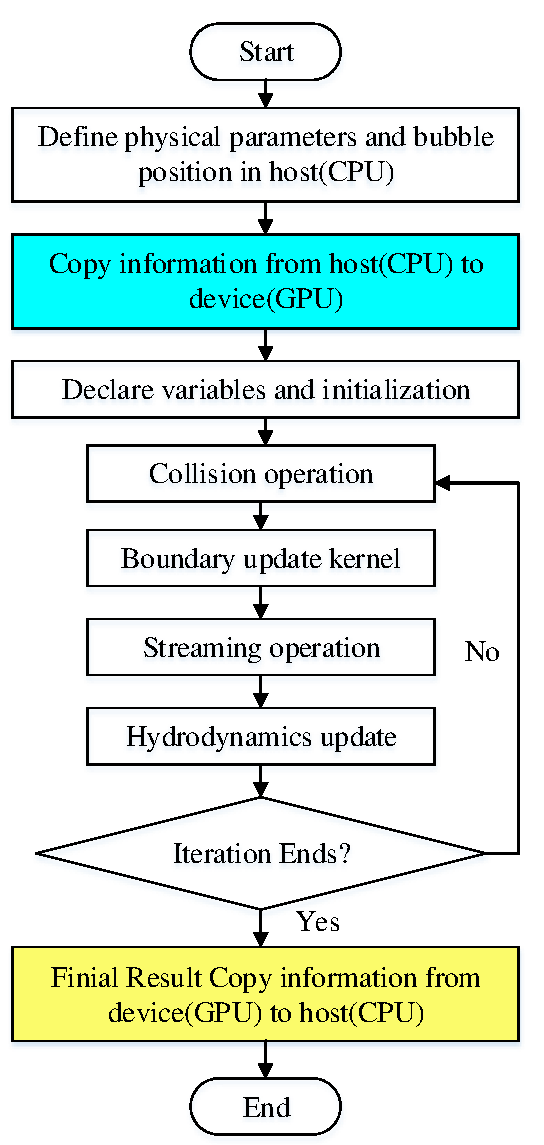
\includegraphics[width=0.4\textwidth]{gpuflow.pdf}
%\vspace{-30pt}
\caption{Flow chart of GPU Implementation}
\label{fig:gpuflow}
%\vspace{-40pt}
\end{wrapfigure}
\setlength{\parindent}{2em} 
The GPU acceleration has been practiced in our research group for a couple years for different research areas such as turbulence\cite{rf:Yu_Chen14_cma}, biomedical flows\cite{rf:Yu15_cf} and porous media flows \cite{rf:Yu_An17_IJHMT,rf:Yu_An17_JPSE}. The general flow chart of GPU implementation is indicated in Fig. \ref{fig:gpuflow}. The difference between GPU parallel and CPU serial is the device used for the LBM implementation.  It is important to combine the feature of GPU with LBM to achieve an efficient GPU-LBM algorithm. Firstly, an A-B (2 sets of distribution functions) pattern is applied before and after streaming to avoid data dependency. Then developed CUDA parallel algorithms are employed in our simulation that includes dynamic allocation, data layout, propagation scheme, register utilization, branch divergence removal, and multi-GPU.  

\subsubsection{Dynamic Allocation} 
By default, the compiled model for a code has a characteristic that the instructions and parameters of the code must be linked in the 2GB static continuous address space. This limitation takes the dominant effect in impeding the simulation of large scale problems. For example, two sets of distribution functions of the lattice Boltzmann model and flow properties in the multi-phase flow, including density, velocity, pressure, chemical potential, and composition are essential arrays to be defined in the CPU host. From the experience of investigating bubble dynamics in a three-dimension (3D) model, the mesh size is around 220$\times$120$\times$220 for our calculations. Due to the limitation of 2GB static continuous address space, the mesh size is up to 280$\times$140$\times$280, which is close to the appropriate mesh size. All these experiences are based on the two bubble coalescence. However, a multiply bubble system, especially with the complex geometry, the needed memory must be larger than 2GB.  Nowadays, a single NVIDIA GPU card has up to 12GB of memory for computing. Hence, it is critical to find a way to release this limitation. Dynamic memory (heap) instead of a static memory (stack) was applied in our simulations.
Dynamic memory (heap) randomly allocates portions from a large pool of memory. The transmission array should be logically contiguous when the data copy between CPU (host) to GPU (device). Hence, in our algorithm, a class of the variable has been developed.
\begin{itemize}
\item The class can dynamically allocate memory in one dimension array, and each variable only uses a total of 5$\times$sizeof(float) or sizeof(double) on the stack. Each variable includes three dimensions in different directions, one variable of fluid properties, and data precision. The illustration likes Array3$<$precision; 3 dimensions in different directions$>$ a variable of fluid property. Take composition C as an example: the class is Array3$<$double; nx; ny; nz$>$ C.  
\item All the other memory is allocated dynamically on the heap in orders in a continuous block through properly overloading the copy constructor. The information which is related to assignment operators will be swap and destroyed.  
\end{itemize}

This class is to manage allocation, deallocation of memory, and utilize the full memory capacity of the GPU cards easily. 

\subsubsection{Propagation Scheme}
Propagation in the LBM relates to streaming. During streaming, there is a problem called misaligned access. There are two main strategies to address this issue in literature as ‘push’ and ‘pull’ algorithms depending on the streaming direction, which is shown in Fig. \ref{fig:PS1} and \ref{fig:PS2} respectively. The streaming direction of the ‘push’ scheme is the same as the usual streaming, which pushes particles from the current cell to the adjacent cells. In other words, it has aligned read and misaligned write in the implementation. The distribution function after the collision is stored in a lattice, as Fig. \ref{fig:PS1}(a) indicates, then the post-streaming values push to the adjacent cell as Fig. \ref{fig:PS1}(b) shows.  Whereas the ‘pull’ scheme has opposite streaming direction, it pulls particles from the adjacent cells to the current cell. In the implementation, it yields to misaligned read and aligned write. The distribution function read from the adjacent cells, as Fig. \ref{fig:PS2}(a) shows. After streaming, the values propagate to the local cell, as Fig. \ref{fig:PS2}(b) illustrates. Since misaligned read is faster than misaligned write in the GPU\cite{rf:Obrecht11}, the ‘pull’ scheme is employed in our simulation.
\begin{figure}[htpb]
\centering
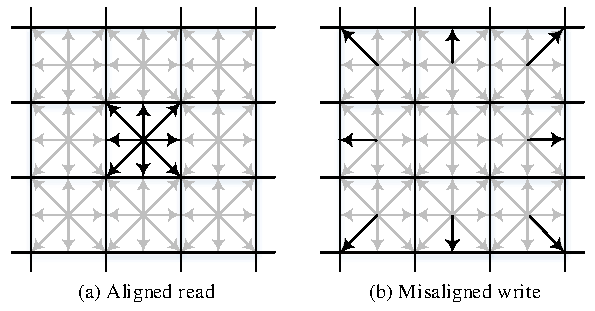
\includegraphics[width=0.72\textwidth]{push.pdf}
\caption{Push scheme for propagation (a) the state before streaming with aligned read (b) the state after streaming with misaligned write}
\label{fig:PS1}
\end{figure}
\begin{figure}[t]
\centering
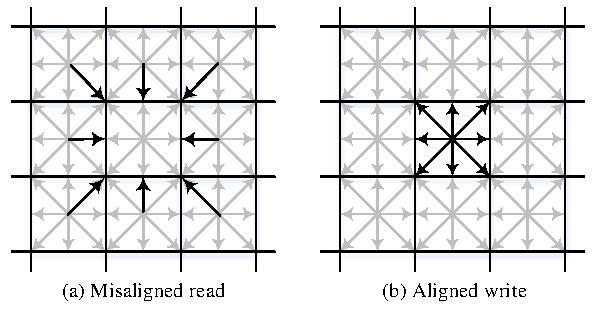
\includegraphics[width=0.72\textwidth]{pull.pdf}
\caption{Pull scheme for propagation (a) the state before streaming with misaligned read (b) the state after streaming with aligned write}
\label{fig:PS2}
\end{figure}
\subsubsection{Data Layout} 
Coalesced memory access is an efficient way to reduce the memory latency of a GPU program that results in acceleration. Coalesced memory access means all the threads in a block access memory address at the same time. Hence, the multiple dimensions arrays are expanded into one dimension arrays. We take the D3Q27 model and assume the mesh size $nx\times ny\times nz$ to show the data layout in the GPU. Regularly, the distribution function stores as 4D array on the CPU such as $f[x][y][z][i]$. Here x, y, z represent the space; i ranges from 0 to 26.  Different structures of one-dimensional arrays in the GPU leads to different effects in the GPU acceleration. There are two main schemes for data layout: Array of Structure (AoS) and Structure of Array (SoA). 
\begin{itemize}
\item Array of Structure (AoS)\\
Twenty-seven distributions of each cell are arranged 27 consecutive elements of the 1D array illustrated in the top panel of Fig. \ref{fig:layout}. The one dimension array format is $f[z\times ny\times nx\times $27$+y\times nx\times$ 27$+z\times$ 27$+i]$. This schema is preferred in the CPU parallelization.
\item Structure of Array (SoA)\\
The value of one distribution of all cells in whole computational domain occupies consecutive elements in memory, which is indicated in the bottom panel of Fig. \ref{fig:layout}. The distribution functions are addressed as $f[i\times z\times nz\times ny\times nx+z \times ny\times nx+y\times nx+z]$. In this scheme, the number of the thread of distribution functions within a wrap (32 threads) can access consecutive memory, so it has been reported that the SoA scheme is suitable for the GPU acceleration\cite{rf:Delbosc14}.
\end{itemize}
%\vspace{-15pt}
\begin{figure}[!htbp]
\centering
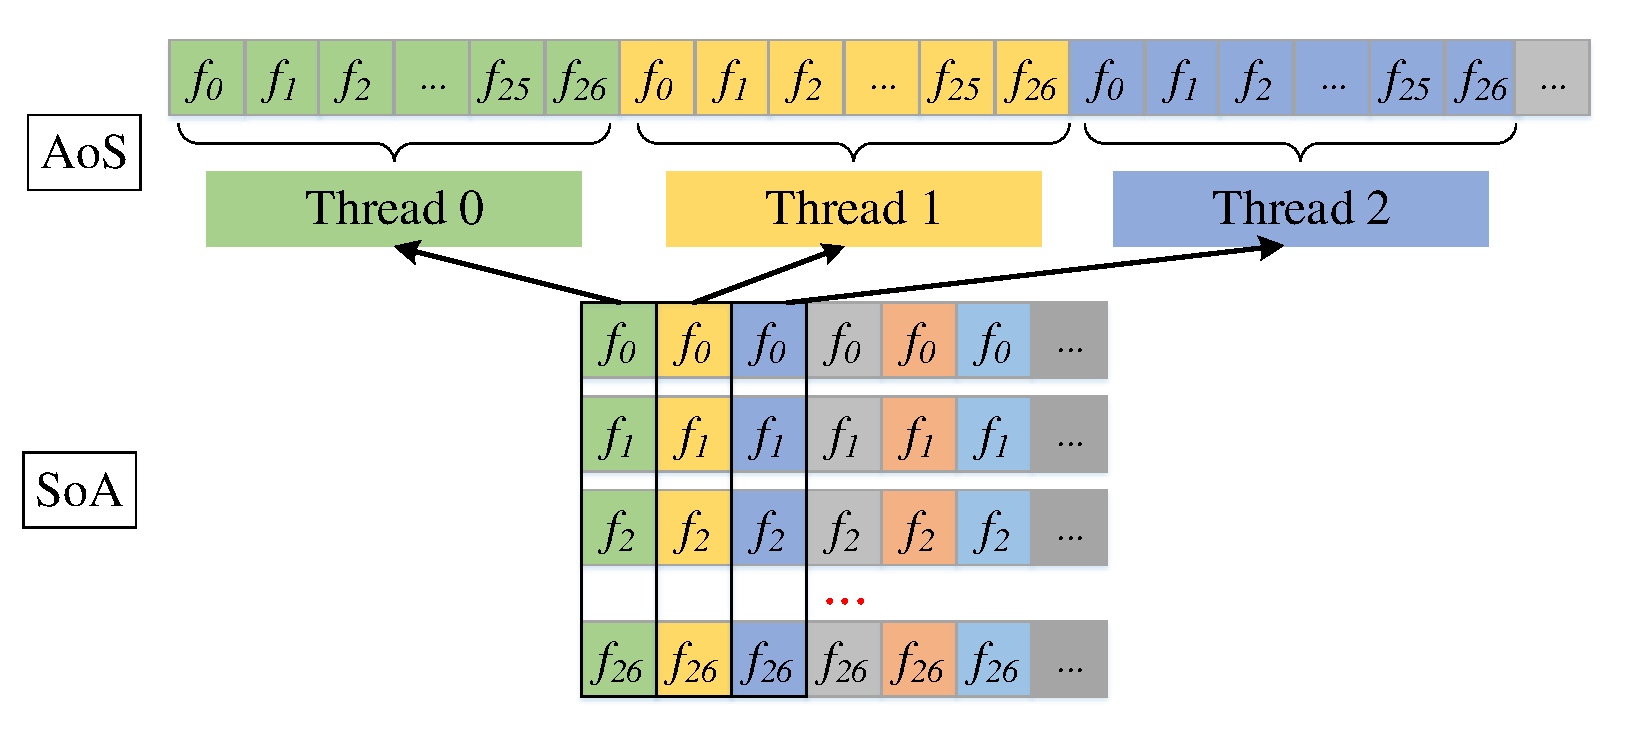
\includegraphics[width=1.0\textwidth]{Structure.pdf}
\vspace{-15pt}
\caption{Data layout: AoS and SoA}
\label{fig:layout}
\end{figure}
%\vspace{-15pt}
\subsubsection{Register Utilization}
CUDA provides a memory hierarchy, including device memory and on-chip memory. Our attention is mainly on the global memory, register, shared memory, and local memory. Global memory is the main part of the device memory, which has a large storage memory and a high latency of 400--600 cycles\cite{rf:Power14}. The register is a kind of on-chip resource distributed to each thread, which has nearly zero cycle latency. But the number of registers may limit the number of concurrent threads on each SM. Similar to the register; shared memory can be fast accessed but limited by its upper bound of storage. When registers or shared memory spills, the extra data will be stored in local memory.  The latency of this type of memory is similar to global memory. 

In these kinds of conditions, register memory is better to be applied in the optimization due to the low latency. Whereas the amount of registers is limited, a single streaming multiprocessor contains 65,536 registers for Tesla K20, and the memory for each register is 32-bit. While too many registers are assigned in each thread, it can’t take full utilization in the memory. For example, 44 registers are needed in the D3Q27 per thread and 1024 threads in one block. 44K registers will be used in one block. In this case, the remaining 21K registers are unused, and only one block is applied in the simulation, then the registers get approximate 60\% utilization. The utilization of register memory effectively in each thread is critical in GPU optimization. The selection of the grid and block size is a scheme to get higher register memory utilization. 
\subsubsection{Branch Divergence Removal}
During the execution, all 32 threads inside one block sequentially compose a warp. When one warp of threads is waiting for data transfer, other warps, which are ready for executing instructions, would be selected out and executed. Therefore the time spent for computation and data access can be overlapped, leading to latency hiding. For execution, CUDA adopts single instruction with multiple threads of architecture where groups of up to eight threads will execute the same instruction in a thread processing array. If the threads inside a warp are not on the same executive path, some data dependence of the if-else branch will be involved. In this case, the implementation of different branches has to be serialized. The update of boundary condition is realized in another kernel to avoid using if-statements. Due to the stretch direction changes at the boundary, the choice of block size will be changed.

%
\subsubsection{Multi-GPU}
\begin{wrapfigure}{R}{0.5\textwidth}
%\vspace{-15pt}
\centering
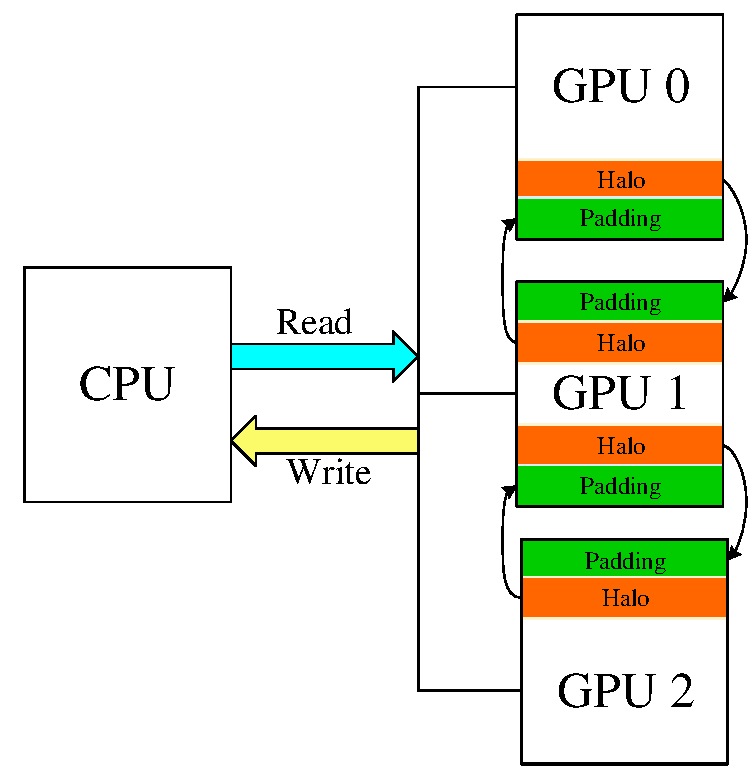
\includegraphics[width=0.5\textwidth]{multigpu.pdf}
\caption{A schematic of data transfer between GPUs}
\label{fig:multigpuflow}
\vspace{-15pt}
\end{wrapfigure}
The multi-GPU part of my research is in the infant stage. Current programming is based on the basic idea of the multi-GPU. However, the performance improvement of the GPU acceleration is obvious in the problems which need high resolution. The basic idea of the multi-GPU is splitting the total memory into several parts, which depends on the number of GPU cards, and then read and written with these cards. Before doing the multi-GPU parallel, two properties of the device should be checked. Firstly,  can the device be able to do peer to peer communication (P2P)? And then, how many GPU cards can be applied in a calculation? As Fig. \ref{fig:multigpuflow} shows, there are three computational data regions in each GPU card, including internal (white region), halo (orange region), and padding part (green region). First, compute the internal and halo parts in a stream, then exchange halo data between neighboring GPUs in a different stream to update the data in different GPU devices. For example, the halo regions in GPU 0 will be transferred to the beginning padding part of GPU 1, and the padding part in the GPU 0 will get the information in the halo regions in the GPU 1. Next, synchronize computation on all devices before proceeding to the next iteration by the function of \textit{cudaDeviceSynchronize()}. Last, the data from all the devices will be written in the CPU part ignore the padding part.
\section{Application studies}
\label{sec:application}
In order to study the bubble dynamics for the coalescence-induced bubble detachment, the computational model is schematized in Fig. \ref{fig:schematic}. Two micro oxygen bubbles (gray color) with the large radius $R_F$ and a small radius $R_M$ in the hydrogen peroxide solution merge into one single bubble (gray color with red color outline) with radius $R_e$. The density and viscosity of oxygen and hydrogen peroxide are $\rho_{O_2}=1.3kg/m^3$,  $\rho_{H_2O_2}=1060kg/m^3$, $\eta_{O_2}=1.92\times 10^{-5}kg/(m\cdot s)$, $\eta_{H_2O_2}=1.06\times 10^{-3}kg/(m\cdot s)$ respectively. The numerical study is conducted in a cuboid domain with height $H=144$($\mu m$), length of the channel $L$ $264 \mu m$, and the width of the channel $W$ the same as the length. For top and bottom sides, boundary conditions shown in Sec.\ref{sec:boundary} is imposed. The periodic boundary is used on the remaining four sides.
\begin{figure}[!htpb]
  \centering
  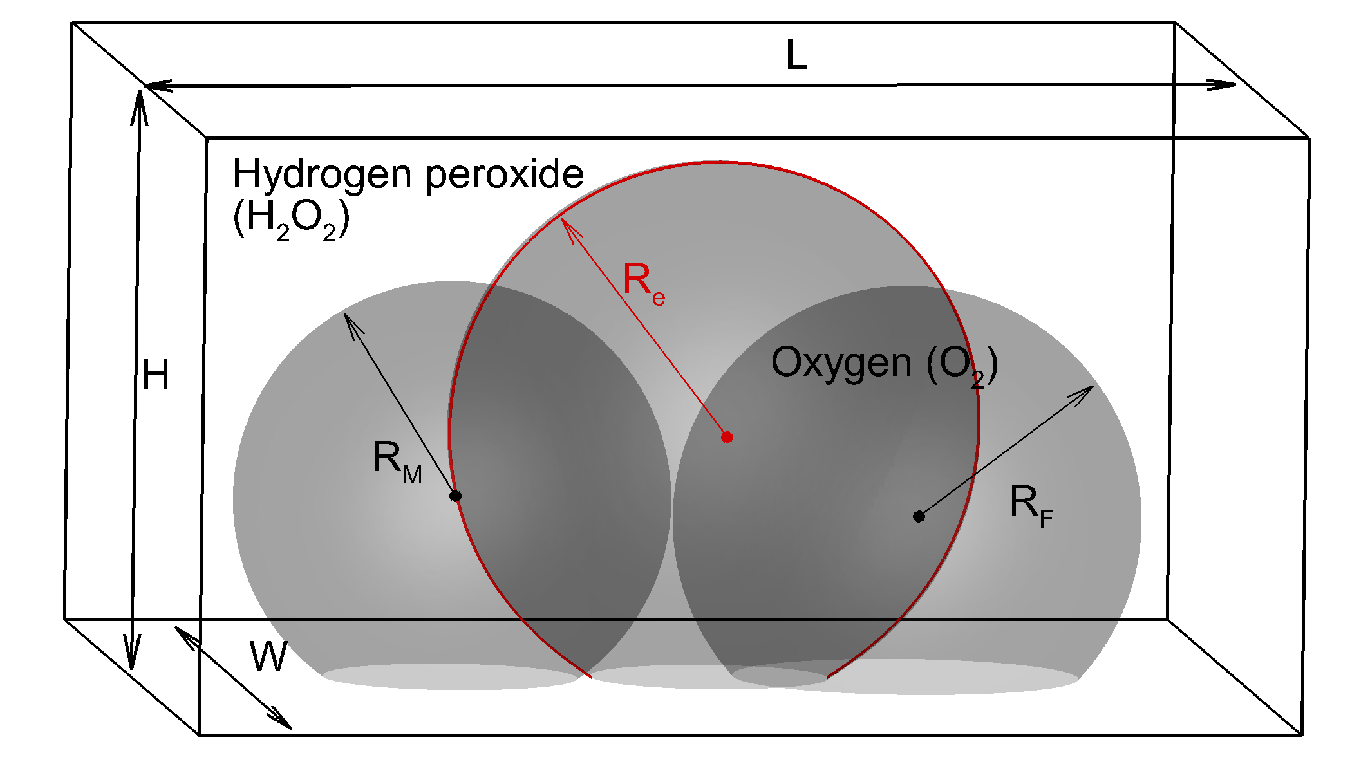
\includegraphics[width=0.5\textwidth]{Schematics.eps}
  \caption{Schematics for coalescence of two micro oxygen bubbles(gray) toward a coalesced bubble (gray with red outline) in the hydrogen solution with a cuboid domain.}\label{fig:schematic}
\end{figure}

\subsection{Convergence check and validation}
Finding the appropriate spatial resolution for the numerical analysis is the first step. Here, we simulate the contact angel when the bubble with $R_{\alpha^{initial}=90^\circ} =60\mu m$ initially sitting on a solid surface,  and the targeted contact angle of the solid surface is $60^\circ$. Fig.\ref{fig:validation}(a) shows the initial bubble (gray color) with half-sphere and the equilibrium state(gray color with the red outline). The simulated contact angle $\alpha^{eq}$ is calculated by Eq.\ref{eq:contactangle} through the measurement of the height of liquid-gas interface $a$ and a base diameter of a bubble $b$ on a solid surface at equilibrium state. The liquid-gas interface which is represented by a contour level $C=0.5$.
\begin{equation}\label{eq:contactangle}
\alpha^{eq}=2arctan(\frac{b}{2a}).
\end{equation}
The convergence check is listed in the Tab.\ref{tab:convergence}. The spatial resolution increases from $44\times24\times 44$ to $264\times144\times 264$ with six different levels, in which the last row shows the spatial convergence. Considering computational cost and accuracy,  we select the spatial resolution of $220\times120\times 220$ to conduct the test.
\begin{table}[!htpb]
\centering
\begin{tabular}{|M{2.5cm}|M{1.3cm}|M{1.3cm}|M{1.4cm}|M{1.4cm}|M{1.5cm}|M{1.5cm}|}
  \hline
  % after \\: \hline or \cline{col1-col2} \cline{col3-col4} ...
  Resolution &$44\times24\times44$ &$88\times48\times88$& $132\times72\times132$& $176\times96\times176$& $220\times120\times220$& $264\times144\times 264$  \\
  \hline
  Simulated contact angle & 53.00 &56.88&58.10&59.22&59.58&59.84\\
 \hline
  Convergence ($\%$) &  & 6.82  &2.10&1.89&0.60&0.43\\
 \hline
\end{tabular}
\caption{Convergence check when the spatial resolution varies from $44\times24\times44$ to $264\times144\times264$ with six levels.}
\label{tab:convergence}
\end{table}

Based on the appropriate resolution, the validation is tested by the case that the initial half-sphere with $60\mu m$ radius on different wetting solid surfaces (different targeted contact angle). Fig.\ref{fig:validation}(b) presents the relationship between the contact angle and dimensionless wetting potential $\Omega_c$ when the contact angle varies from $40^\circ$ and $150^\circ$, the numerical result is well consistent with the analytical result so that the test cases confirm the model is reliable.
\begin{figure}[!htpb]
  \centering
  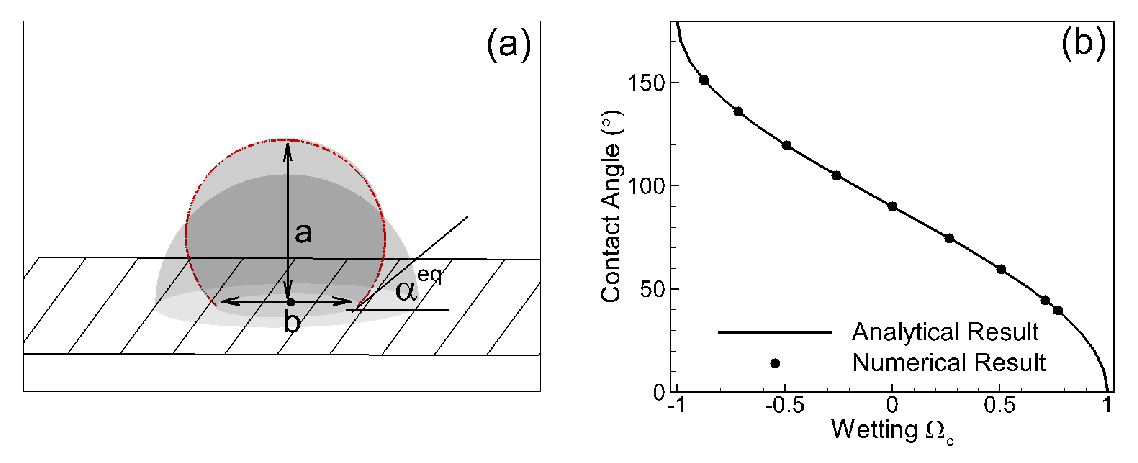
\includegraphics[width=0.9\textwidth]{Validations.eps}
  \caption{(a) Schematics of the half sphere bubble initially sitting on the wetting surface. The slice in the middle of domain of the equilibrium state (gray color with the red outline) is chosen to do the validation. (b) The comparison of the relationship between contact angle and dimensionless wetting potential from analytical and numerical results.  }\label{fig:validation}
\end{figure}
\subsection{Coalescence-induced bubble detachment}
In the microchannel, the gravity compared to surface tension force can be ignored so that bubbles can't easily detach from the surface. They will coalesce and eventually plug the microchannel. Bubble detachment is one of the common phenomena in bubble dynamics which happened in the post-coalescence stage needing a long time to be observed.  The bubble coalescence process shows as Fig.\ref{fig:detach}. It starts from the two touching parent microbubbles  Fig.\ref{fig:detach}(a), the neck bridge is generated and grows Fig.\ref{fig:detach}(b), then bubble oscillate with small amplitude Fig.\ref{fig:detach}(c), (d), (e), (f). 
During the oscillate process, the coalescence-induced detachment of the bubble can be observed as Fig.\ref{fig:detach}(f).   
\begin{figure}[!htpb]
  \centering
  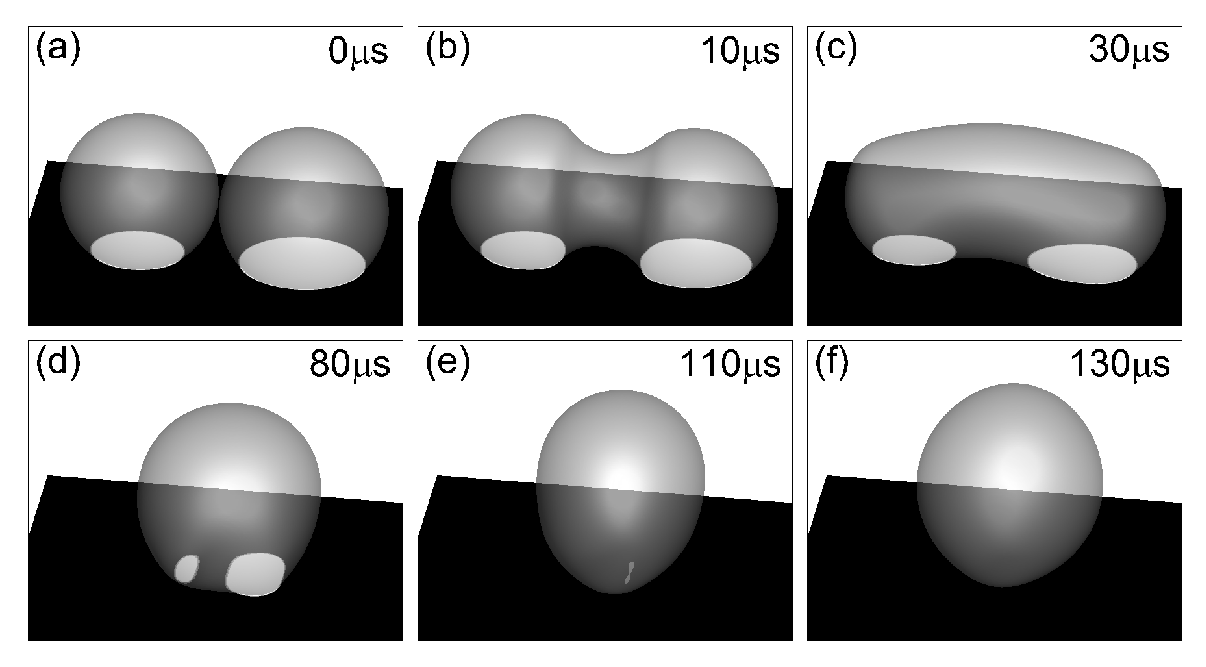
\includegraphics[width=0.95\textwidth]{Process.eps}
  \caption{Time evolution of bubble coalescence}
 \label{fig:detach}
\end{figure}

\subsection{Performance test}
Million lattice updates per second (MLUPS) is a parameter to indicate the computational performance for lattice Boltzmann simulations. To observe the coalescence-induced bubble detachment during two bubbles coalescing in the simulation will spend 44 days when we use the hardware: Broadwell E5-2683 v3@ 2.30GHz CPU. Additionally, massive parameter cases and multi-bubbles system are needed to study the bubble dynamics in the practical problems. Hence, GPU acceleration is critical to be employed in the application case that has high computational cost caused by a large number of cases and high resolution. The performance of our GPU accelerated lattice Boltzmann modeling is tested through single GPU and multi-GPU based on four machines with different types of CPU and GPU cards, as Tab. \ref{tab:machine} shows. We employed the GPU parallel approaches in the same code and tested the speed-up with different machines. 
\begin{table}[!htpb]
\centering
\small
\begin{tabular}{|c|c|c|c|}
  \hline
  % after \\: \hline or \cline{col1-col2} \cline{col3-col4} ...
   & CPU & GPU & GPU number\\
   \hline
1 & Intel(R) Xeon(R) E5645 & Tesla C2050 & 1 \\
  \hline
2 & Intel(R) Xeon(R) X5660& Tesla C2750 & 4\\
\hline 
3 & \multirow{2}{*}{Intel Broadwell E5-2683 v4} &Tesla P100 & 2\\
  \cline{1-1}
  \cline{3-4} 
 4 &   &Tesla K80 & 4\\
  \hline 
\end{tabular}
\caption{Information on the machines used in the computation}
\label{tab:machine}
\end{table}

\begin{itemize}
\item Single GPU\\
 GPU acceleration applied in the application case with five different spatial resolutions $88\times48\times88$, $132\times72\times132$, $176\times96\times176$, $220\times120\times220$, $264\times144\times264$. Here, we use the advancing GPU card P100 (the third machine listed in Tab. \ref{tab:machine}), which is popularly equipped in the supercomputers to do the performance test. The speed-up increases with resolution increases. We can see from Tab. \ref{tab:bubblegpu} the speed-up is 2110 when the appropriate resolution derived from convergence check is selected. In other words, a numerical case can be done within half an hour with parallel execution, whereas it takes 44 days with serial execution.
 \begin{table}[!htpb]
\centering
\begin{tabular}{|c|c|c|c|c|}
  \hline
  % after \\: \hline or \cline{col1-col2} \cline{col3-col4} ...
  Resolution & GPU parallel(MLUPS) &Serial(MLUPS) & Speed-up & Parallel vs. Serial (in hour)    \\
  \hline
  $88\times 48\times 88$ & 181& 0.13 & 1428& 0.02/29\\
  \hline
  $132\times 72\times132$ & 176 & 0.11 &1653 & 0.08/132\\
  \hline
  $176\times96\times 176$ & 200 & 0.11 & 1758& 0.25/439\\
  \hline
  $220\times120\times220$ & 211& 0.10 & 2110&  0.50/1055\\
  \hline
   $264\times144\times264$ &206& 0.10 & 1994&  1.25/2492\\
  \hline
\end{tabular}
\caption{GPU acceleration comparing with the CPU serial performance. The last column is a comparison of parallel vs. serial  wall-clock time for a complete process of coalescence.}
\label{tab:bubblegpu}
\end{table}

Meanwhile, we take the appropriate resolution $220\times120\times220$ to test performance with a single GPU in different machines listed as Tab. \ref{tab:machine}. The result of the performance test is seen in Fig. \ref{fig:machince}. The advancing hardware has faster performance, such as Tesla P100 is 20 times faster than the Tesla C2050/C2750.
\begin{figure}[!htpb]
\begin{minipage}{0.5\textwidth}
  \centering
  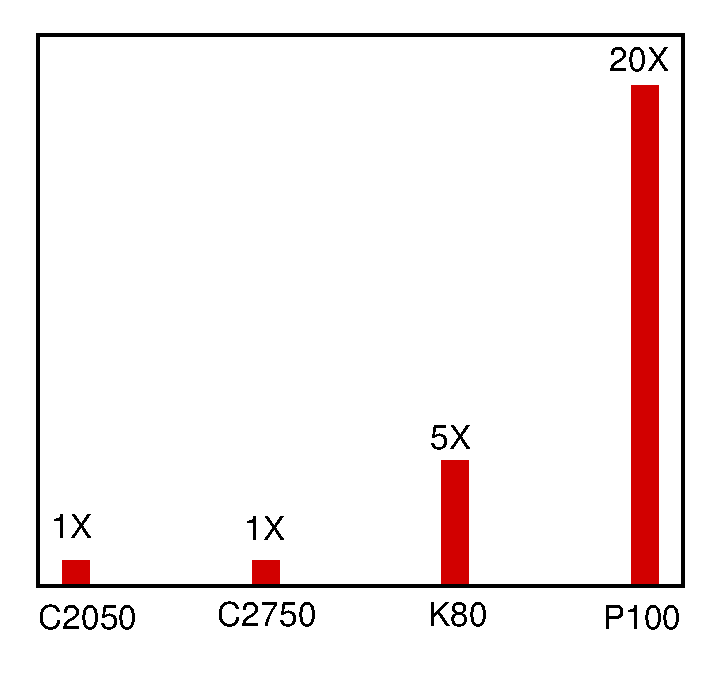
\includegraphics[width=0.9\textwidth]{machince.eps}
  \caption{The performance of the different machine resources listed in the Tab.\ref{tab:machine}}
 \label{fig:machince}
\end{minipage}
\begin{minipage}{0.5\textwidth}
  \centering
  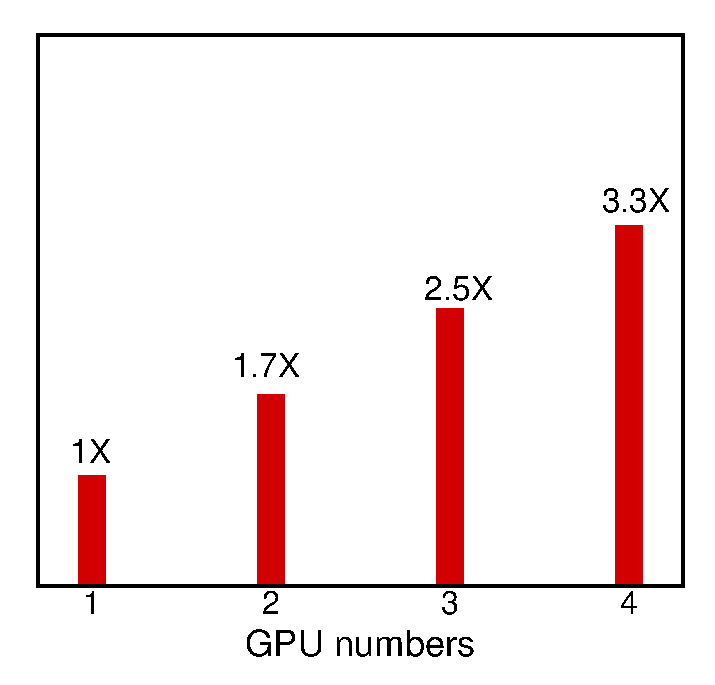
\includegraphics[width=0.9\textwidth]{multigpu.eps}
\caption{Performance of different numbers of GPU card. The performance accelerates as the numbers of GPU card increases.}
\label{fig:multigpu}
\end{minipage}
\end{figure}

\item Multi-GPU\\
Three kinds of four machines listed in Tab. \ref{tab:machine} can be used to do the multi-GPU parallelism. Considering the number of GPU cards and the fastest performance of GPU cards, we use Tesla K80 (machine 4) to perform the efficiency of the algorithm of multi-GPU. Fig \ref{fig:multigpu} exhibits the GPU acceleration with the spatial resolution 220$\times$120$\times$220 by one, two, three, four GPU cards separately. The performance is accelerating when the number of GPU cards increases.  
\end{itemize}

\section{Summary $\&$ Future Work}
\label{sec:Sum}
In this paper, we want to perform the capability and efficiency of our GPU accelerated lattice Boltzmann modeling that imposes a gas-liquid-solid interface to study the bubble dynamics. First, to perform the capability, we validate a half-sphere bubble sitting on the different wetting surfaces with a targeted contact angle from $40^\circ$ to $150^\circ$. In the bubble dynamics problems, the speed accelerated is critical due to the high computational cost caused by the massive parameter cases and fine resolution. Then the efficiency of GPU accelerated lattice Boltzmann modeling is tested by the coalescence-induced bubble detachment phenomena when two parent oxygen bubbles in the hydrogen peroxide solution attached in the Pt surface, which the targeted contact angle is $ 36^\circ$. From the test, the performance of the lattice Boltzmann modeling is increasing up to 2110, 6963 by single GPU, 4 GPU cards accelerated, respectively. For the current application case, we use it to study the bubble dynamics, the efficiency of the modeling is enough. However, in large scale problems such as multiply bubbles system, arbitrary geometry, and so on, the efficiency of the modeling needs improving. There are many approaches we want to develop in the future: 1. Optimize the multi-GPU algorithm, especially on the part of data transformation and distribution; 2. Develop the approach that MPI, OpenMP combines with GPU parallelism with one node and multi-nodes.     

\section*{Acknowledgments}
This research is supported by the graduate assistantship from School of Engineering and Technology. And this work used the Extreme Science and Engineering Discovery Environment (XSEDE), which is supported by National Science Foundation grant number ACI-1053575.
%% The Appendices part is started with the command \appendix;
%% appendix sections are then done as normal sections
%% \appendix

%% \section{}
%% \label{}

%% If you have bibdatabase file and want bibtex to generate the
%% bibitems, please use
%%
%%  \bibliographystyle{elsarticle-num}
%%  \bibliography{<your bibdatabase>}

%% else use the following coding to input the bibitems directly in the
%% TeX file.

%\begin{thebibliography}{00}
%
%%% \bibitem{label}
%%% Text of bibliographic item
%
%\bibitem{}
%
%\end{thebibliography}
%\renewcommand{\refname}{References}
\bibliographystyle{elsarticle-num}
%\section*{\refname}
\bibliography{reference, ReferenceIntroduction}

\end{document}
\endinput
%%
%% End of file `elsarticle-template-num.tex'.
